\documentclass[11pt]{article}
\usepackage{amsmath, amsthm, amssymb, pdfpages} 
\usepackage{fullpage}
\usepackage{hyperref}
\usepackage{graphicx}
\usepackage[capitalize]{cleveref}

\usepackage{pdfpages} % Required to include PDFs


% next three for UTF8 to work (for non-ASCII names to work without awkward codes)
\usepackage[T1]{fontenc}
\usepackage{textcomp}
\usepackage[utf8]{inputenc}

% import biblatex with prefered settings
% loads biblatex with all the nice standard options that John determined some time ago!
% this version uses a ``Harvard'' style (first author last name, year in parentheses).
% also loads xpatch

% biblatex
% harvard style
\usepackage[style=authoryear,natbib,maxcitenames=2,doi=false,isbn=false,url=false,backend=bibtex]{biblatex}
% % numeric style
% \usepackage[style=numeric-comp,sorting=none,giveninits=true,doi=false,isbn=false,url=false,backend=bibtex]{biblatex}
% % to have citep etc work without a hitch here...
% \newcommand{\citep}{\cite}
% \newcommand{\citet}{\cite}

% remove "In: " before journal title
\renewbibmacro{in:}{}
% remove language
\AtEveryBibitem{\clearlist{language}}
% remove month
\AtEveryBibitem{\clearfield{month}}
% and also notes
\AtEveryBibitem{\clearfield{note}}
% remove dots between volume and issue
\usepackage{xpatch}
\xpatchbibmacro{volume+number+eid}{%
  \setunit*{\adddot}%
}{%
}{}{}
% put issue in parentheses
\DeclareFieldFormat[article]{number}{\mkbibparens{#1}}

\bibliography{zotero} % biblatex wants this in the preamble...

% path for figures
\graphicspath{ {../} }

\usepackage[noT]{kinshipsymbols}
% % copy of \Fst from package `kinshipsymbols`

\newcommand{\beginsupplement}{%
  \setcounter{table}{0}
  \renewcommand{\thetable}{S\arabic{table}}%
  \setcounter{figure}{0}
  \renewcommand{\thefigure}{S\arabic{figure}}%
  \setcounter{section}{0}
  \renewcommand{\thesection}{S\arabic{section}}%
  \setcounter{equation}{0}
  \renewcommand{\theequation}{S\arabic{equation}}%
  \setcounter{page}{1}
  \renewcommand{\thepage}{S\arabic{page}}%
}



% some more definitions
\newcommand{\kinMat}{%
  \ensuremath{%
    \mathbf{\Phi}
  }%
  \xspace%
}%
\newcommand{\kinMatStdLim}{%
  \ensuremath{%
    \mathbf{\hat{\Phi}}^\text{std-lim}
  }%
  \xspace%
}%

\newcommand{\kinMatEstNamed}[1]{%
  \ensuremath{%
    \mathbf{\hat{\Phi}}^\text{#1}
  }%
  \xspace%
}%

% for theorems!
\usepackage{amsthm}
%\newtheorem{thm}{Theorem}[section]
\newtheorem*{thm}{Theorem}
%\newtheorem{lem}[thm]{Lemma}
\newtheorem*{lem}{Lemma}
% \newtheorem{lemma}[theorem]{Lemma}

% % double line spacing (PLoS wants this)
% \usepackage{setspace}
% \doublespacing
% spacing smaller than double
\renewcommand{\baselinestretch}{1.2}

\title{\Large \textbf{Kinship estimation bias carries over to heritability estimation bias using variance components}}
\author{Zhuoran Hou$^1$, Alejandro Ochoa$^{1,2,*}$}
\date{}

\begin{document}
\maketitle

\noindent
$^1$ Department of Biostatistics and Bioinformatics, Duke University, Durham, NC 27705, USA \\
$^2$ Duke Center for Statistical Genetics and Genomics, Duke University, Durham, NC 27705, USA \\
$^*$ Corresponding author: \texttt{alejandro.ochoa@duke.edu}


\begin{abstract}
Heritability is a fundamental parameter of diseases and other traits, quantifying the contribution of genetics to that trait as opposed to non-genetic environmental factors. Heritability is reflected in the extent to which relatives have similar phenotypes. The estimation of kinship matrices, also known as Genetic Relatedness Matrices or “GRMs”, is required for heritability estimation with many common approaches based on variant components. However, the most common “standard” kinship estimator employed by these approaches, including the popular GCTA package, can be severely biased in structured populations. In this study, we first characterize the theoretically predicted heritability estimation bias in the GCTA model due to kinship bias. Heritability estimation in this model requires unbiased estimates of the random effect coefficient, which we find is biased when the standard kinship estimator is used, and this bias depends only on the mean kinship value and the true heritability. We conduct simulation studies to evaluate heritability estimation with various kinship matrices for scenarios such as admixture structure only and admixture plus family structure. The simulation results validate our theoretical prediction of the bias of the standard GCTA approach and show that our unbiased kinship matrices result in unbiased heritability estimates. A further complication is that upweighting rare variants in these kinship estimates, which is common practice, introduces an additional bias that has not been characterized in closed form.  Then we apply various kinship matrices to several real datasets, such as the San Antonio Family Study, the Hispanic Community Health Study / Study of Latinos, and a Nephrotic Syndrome multiethnic cohort, to further characterize the source of biases and illustrate their extent in practice. We find that the heritability estimations using our unbiased kinship matrices lead to higher values, which are more consistent with previously published estimates in unstructured populations. Overall, we find that the most commonly used kinship estimators bias heritability estimates downward when population structure is present, whereas using unbiased kinship estimators can address this source of bias.
\end{abstract}

% \clearpage

% \tableofcontents

\clearpage
	
\section{Introduction}

Heritability is an important parameter of diseases and other traits, quantifying the contribution of genetics to that trait as opposed to non-genetic environmental factors \citep{lush1949heritability}. Heritability is reflected in the extent to which relatives have similar phenotypes \citep{visscher2008heritability}. In addition, heritability is closely related to the polygenic risk score (PRS) method, an estimate of genetic liability to a trait for individuals, as it defines the upper bound of the performance of PRS \citep{choi2020tutorial}. 

Heritability has long been estimated from close relatives, such as twins or siblings \citep{falconer1996introduction}, or more complex pedigrees \citep{almasy_multipoint_1998}. The variance component model of the SOLAR approach, which is based on estimating kinship from pedigrees, enables the use of more distant relatives \citep{almasy_multipoint_1998}. GCTA extended the last approach to population data, which was used to demonstrate that SNPs likely explain the majority of missing heritability for height \citep{yang_common_2010,yang_gcta:_2011}. Alternative approaches for estimating heritability, such as LD Score Regression \citep{bulik2015ld,luo2021estimating} and SumHer \citep{speed2019sumher}, work with GWAS summary data and enable partitioning heritability within gene sets. 

Accurate kinship estimation is crucial for heritability estimation based on LMMs, such as GCTA. However, the most common kinship estimator employed by these approaches can be severely biased in structured populations \citep{ochoa_estimating_2021}. Previous study showed, empirically and theoretically, that association tests are invariant to the use of common biased kinship estimators compared with an unbiased estimator \citep{hou2023genetic}. However, heritability estimation requires unbiased estimates of the random effect coefficient, which is biased when the standard kinship estimator is used. 

In this study, we first characterize the theoretically predicted heritability estimation bias due to kinship bias, following the derivation in the previous study. We conduct simulation studies to evaluate heritability estimation with various kinship matrices for scenarios such as admixture structure only and admixture plus family structure. Then we apply various kinship matrices to several real datasets to further characterize the source of biases and their extent.


\section{Methods}

\subsection{Genetic model}

Suppose that there are $m$ biallelic loci and $n$ diploid individuals.
The genotype $\xij \in \{0,1,2\}$ at a locus $i$ of the individual $j$ is encoded as the number of reference alleles, for a pre-selected but otherwise arbitrary reference allele per locus.
\kt is the kinship coefficient of two individuals $j$ and $k$, and \pit is the ancestral allele frequency at locus $i$, then under the kinship model \citep{malecot_mathematiques_1948, wright_genetical_1949, jacquard_structures_1970, astle_population_2009, ochoa_estimating_2021} the expectation and covariance are given by
\begin{equation}
  \label{eq:model0}
  \E \left[ \mathbf{x}_i  \right]
  =
    2 \pit \mathbf{1}
  ,
  \quad\quad
  \Cov \left(\mathbf{x}_i  \right)
  =
    4 \pit \left( 1 - \pit \right) \kinMat
    ,
\end{equation}
where $\mathbf{x}_i = (\xij)$ is the vector of genotypes at locus $i$, $\kinMat = (\kt)$ is the $n \times n$ kinship matrix, and $\mathbf{1}$ is a vector of ones.


The quantitative trait vector $\mathbf{y}$ for all individuals is assumed to follow a linear polygenic model,
\begin{equation}
  \label{eq:trait}
  \mathbf{y}
  =
  \mathbf{1}_n \alpha + \mathbf{X}' \mathbf{\beta}  + \mathbf{\epsilon},
\end{equation}
where $\alpha$ is the intercept, $\mathbf{\beta} = (\beta_i)$ is a vector of genetic effect coefficients for each locus $i$, and $\mathbf{\epsilon}$ is a vector of non-genetic effects.

Let us shift the mean of genotypes to the intercept and denote $\mathbf{s}=\mathbf{X}' \mathbf{\beta}$, then:
\begin{align*}
     \mathbf{y}  &=
  \mathbf{1}_n \alpha + \mathbf{s}  + \mathbf{\epsilon},
   \\
  \mathbf{s} 
    \sim
    \text{Normal} \left( \mathbf{0}, 2 \sigma^{2}_g \kinMat \right), \quad
    \mathbf{\epsilon} &
    \sim
    \text{Normal} \left( \mathbf{0}, \sigma^{2}_e \mathbf{I}_n  \right), 
    \mathbf{s}  + \mathbf{\epsilon} 
    \sim
    \text{Normal} \left( \mathbf{0}, 2 \sigma^{2}_g \kinMat +  \sigma^{2}_e \mathbf{I}_n  \right).
\end{align*}

To analyze the covariance structure of the trait, we treat $\alpha$ and $\mathbf{\beta}$ as fixed parameters, while $\mathbf{X}$ and $\mathbf{\epsilon}$ are random.
The non-genetic effects are assumed to be independent with variance $(1-h^2) \sigma^2$ given by the total trait variance scale $\sigma^2$ and the narrow-sense heritability $h^2$:
\begin{align*}
  \E[\mathbf{\epsilon}]
  =
  \mathbf{0}_n
  ,
  \quad\quad
  \Cov(\mathbf{\epsilon})
  =
   \sigma^{2}_e \mathbf{I}_n
  ,
  \\
    \mathbf{X}' \mathbf{\beta}  + \mathbf{\epsilon}
    \sim
    \text{Normal} \left( \mathbf{0}, 2 \sigma^{2}_g \kinMat +  \sigma^{2}_e \mathbf{I}_n  \right).
\end{align*}
Then the narrow-sense heritability $h^2$ is defined as:
\begin{align*}
    h^{2}  =
    \frac{
    \sigma^{2}_g
    }{
    \sigma^{2}_g + \sigma^{2}_e
    }.
\end{align*}

\subsection{Kinship estimation}
Each estimator bias type has two locus weight types called \textit{ratio-of-means} (ROM) and \textit{mean-of-ratios} (MOR) \citep{bhatia_estimating_2013, ochoa_estimating_2021}.
Only ROM estimators have closed-form limits.
Below
$
\pith
=
\frac{1}{2n} \mathbf{x}_i' \mathbf{1}
$
is the standard ancestral allele frequency estimator,
where the prime ($'$) denotes matrix transposition,
and
$\kinMatEstNamed{name} = (\ktHatNamed{name})$
relates the scalar and matrix formulas of each named kinship estimator.
\subsubsection{Standard kinship estimator}

The ``standard'' kinship estimator is the most widely used estimator in various applications of population structure \citep{astle_population_2009, speed_relatedness_2015, wang_efficient_2017}, including
heritability estimation \citep{speed_improved_2012, speed_relatedness_2015, speed_reevaluation_2017}
and genetic association tests based on PCA \citep{price_principal_2006},
LMM \citep{astle_population_2009, zhou_genome-wide_2012, loh_efficient_2015, sul_population_2018},
and other models \citep{rakovski_kinship-based_2009, thornton_roadtrips:_2010}.
The popular heritability estimation approach GCTA \citep{yang_common_2010, yang_gcta:_2011} employs a variant of this estimator that is detailed in the next paragraph.


The ROM and MOR versions of the standard kinship estimator are, respectively,

\begin{align}
  \label{eq:kinship_std_rom}
  \ktHatNamed{std-ROM}
  &=
    \frac{
    \sum\limits_{i=1}^m \left( \xij - 2 \pith \right) \left( \xij[k] - 2 \pith \right)
    }{
    \sum\limits_{i=1}^m 4 \pith \left( 1-\pith \right)
    }
    , \\
  \label{eq:kinship_std_mor}
  \ktHatNamed{std-MOR}
  &=
    \frac{1}{m} \sum\limits_{i=1}^m \frac{\left( \xij - 2 \pith \right) \left( \xij[k] - 2 \pith \right)}{4 \pith \left( 1-\pith \right)}    .
\end{align}

The ROM estimator has a biased limit, which is a function of the true kinship matrix \citep{ochoa_estimating_2021}:
\begin{equation}
  \label{eq:kinship_std_lim}
  \kinMatEstNamed{std-ROM}
  \toas
    \frac{1}{1 - \bar{\varphi}}
  \left(
    \kinMat
    + \bar{\varphi} \mathbf{J}
    - \boldsymbol{\varphi} \mathbf{1}' 
    - \mathbf{1} \boldsymbol{\varphi}' 
  \right)
  ,
\end{equation}
where
$\mathbf{J} = \mathbf{1} \mathbf{1}'$ is the $n \times n$ matrix of ones,
$\boldsymbol{\varphi} = \frac{1}{n} \kinMat \mathbf{1}$ is a vector of per-row mean kinship values, and
$\bar{\varphi} = \frac{1}{n^2} \mathbf{1}' \kinMat \mathbf{1}$ is the scalar overall mean kinship.
The MOR estimator does not have a closed-form limit, but it is well approximated by Eq. (\ref{eq:kinship_std_lim}) in practice, especially when loci with small minor allele frequencies are excluded prior to calculating this estimate.

\subsubsection{Popkin kinship estimator}
The popkin (population kinship) estimator \citep{ochoa_estimating_2021}, generalized here to include locus weights $w_i$, is given by
\begin{equation}
  \label{eq:popkin}
  \ktHatNamed{popkin}
  =
  1 - \frac{\Ajk}{\AMinHat}
  , \quad\quad
  \Ajk
  =
  \frac{1}{m} \sum_{i=1}^m w_i ( (\xij-1)(\xij[k]-1) - 1 )
  ,
\end{equation}
where in this work $\AMinHat = \min_{j \ne k} \Ajk$, and $w_i$ must be positive but need not add to 1.
We consider two broad forms for this estimator.
The original ROM estimator has $w_i = 1$ and has an unbiased almost sure limit as the number of loci $m$ goes to infinity,

$$
\kinMatEstNamed{popkin-ROM} \toas \kinMat,
% \ktHatNamed{popkin-ROM} \toas \kt,
$$
under the assumption that the true minimum kinship is zero.
The MOR version, introduced here, outweighs rare variants using $w_i = \left( \pith \left( 1 - \pith \right) \right)^{-1}$; although it does not have a closed-form limit, it is approximately unbiased as well and is connected to the most common estimator, the standard MOR \citep{hou2023genetic}. 

\subsection{Heritability estimation bias due to kinship bias}
\label{Estimation bias}

In our recent work, we characterized the theoretical relationship between variance component estimates of a biased kinship matrix and its unbiased counterpart \citep{hou2023genetic}.
For standard ROM estimator, 
\begin{align*}
  \label{eq:kin-std-lim-C}
  \kinMatEstNamed{std-ROM}
  =
  \frac{1}{1 - \bar{\varphi}}
  \mathbf{C} \kinMat \mathbf{C}  ,
\end{align*}
where $ \mathbf{C} = \mathbf{I} - \frac{1}{n} \mathbf{J}$ is the centering matrix.
Let the estimates derived from the unbiased kinship matrix be $\hat{\sigma}^2_g, \hat{\sigma}^2_e$, so that the heritability estimate is
\begin{align*}
  \hat{h}^2
  &=
    \frac{
    \hat{\sigma}^2_g
    }{
    \hat{\sigma}^2_g + \hat{\sigma}^2_e
    }
  .
\end{align*}
Now, denote the estimates derived from the biased kinship matrix as
$\hat{\sigma}^{2,\text{biased}}_g, \hat{\sigma}^{2,\text{biased}}_e$.
Then, the model based on the biased kinship matrix is:
\begin{align*}
\mathbf{y}  &=
  \mathbf{1}_n \alpha ^{\text{biased}} + \mathbf{s}^{\text{biased}}  + \mathbf{\epsilon},
  \\
  \mathbf{s}^{\text{biased}} &= \mathbf{C} \mathbf{s}
  \sim
  \text{Normal} \left( \mathbf{0}, 2 \hat{\sigma}^{2,\text{biased}}_g \kinMatEstNamed{std-ROM} \right),
  \\
  \mathbf{s}^{\text{biased}} &= \mathbf{s} - \mathbf{1}_n \bar{\mathbf{s}},
  \quad
  \alpha ^{\text{biased}}=\alpha+ \bar{\mathbf{s}} ,
  \quad
    \bar{\mathbf{s}}\sim
  \text{Normal} \left( 0,  \hat{\sigma}^{2}_g \bar{\varphi} \right),
\end{align*}
and we found that the relationship between these estimates is algebraically given by
\begin{align*}
  \hat{\sigma}^{2,\text{biased}}_g
  &=
    (1 - \bar{\varphi}) \hat{\sigma}^2_g
    , \\
  \hat{\sigma}^{2,\text{biased}}_e
  &=
    \hat{\sigma}^2_e
    ,
\end{align*}
where $\bar{\varphi}$ is the mean value of the unbiased kinship matrix \citep{hou2023genetic}.
Therefore, after noting that
\begin{align*}
  % \hat{h}^2 ( \hat{\sigma}^2_g + \hat{\sigma}^2_e )
  % &=
  %   \hat{\sigma}^2_g
  %   , \\
  % \hat{\sigma}^2_e
  % &=
  %   \hat{\sigma}^2_g \frac{ 1 - \hat{h}^2 }{ \hat{h}^2 }
  %   , \\
  \hat{\sigma}^2_e
  &=
    \left( \frac{ 1 }{ \hat{h}^2 } - 1 \right) \hat{\sigma}^2_g 
    ,
\end{align*}
and substituting this and the values of the biased parameters, we find a form for the biased heritability estimate in terms of the unbiased estimate and the mean kinship:
\begin{align*}
  \hat{h}^{2,\text{biased}}
  &=
    \frac{
    \hat{\sigma}^{2,\text{biased}}_g
    }{
    \hat{\sigma}^{2,\text{biased}}_g + \hat{\sigma}^{2,\text{biased}}_e
    }
  \\
  &=
    \frac{
    (1 - \bar{\varphi}) \hat{\sigma}^2_g
    }{
    (1 - \bar{\varphi}) \hat{\sigma}^2_g
    + \left( \frac{ 1 }{ \hat{h}^2 } - 1 \right) \hat{\sigma}^2_g 
    }
  \\
  &=
    \hat{h}^2
    \frac{
    1 - \bar{\varphi}
    }{
    1 - \bar{\varphi} \hat{h}^2
    }
    .
\end{align*}
We further plot this relationship between the true heritability and biased estimates in \cref{fig:h}. From this, we found that the bias becomes larger for the heritability ranging from 0.5 to 0.8 approximately while decreasing to 0 when the heritability is close to 0 or 1. In addition, the bias increases when $\bar{\varphi}$ increases.
\begin{figure}[bp!]
  \centering
  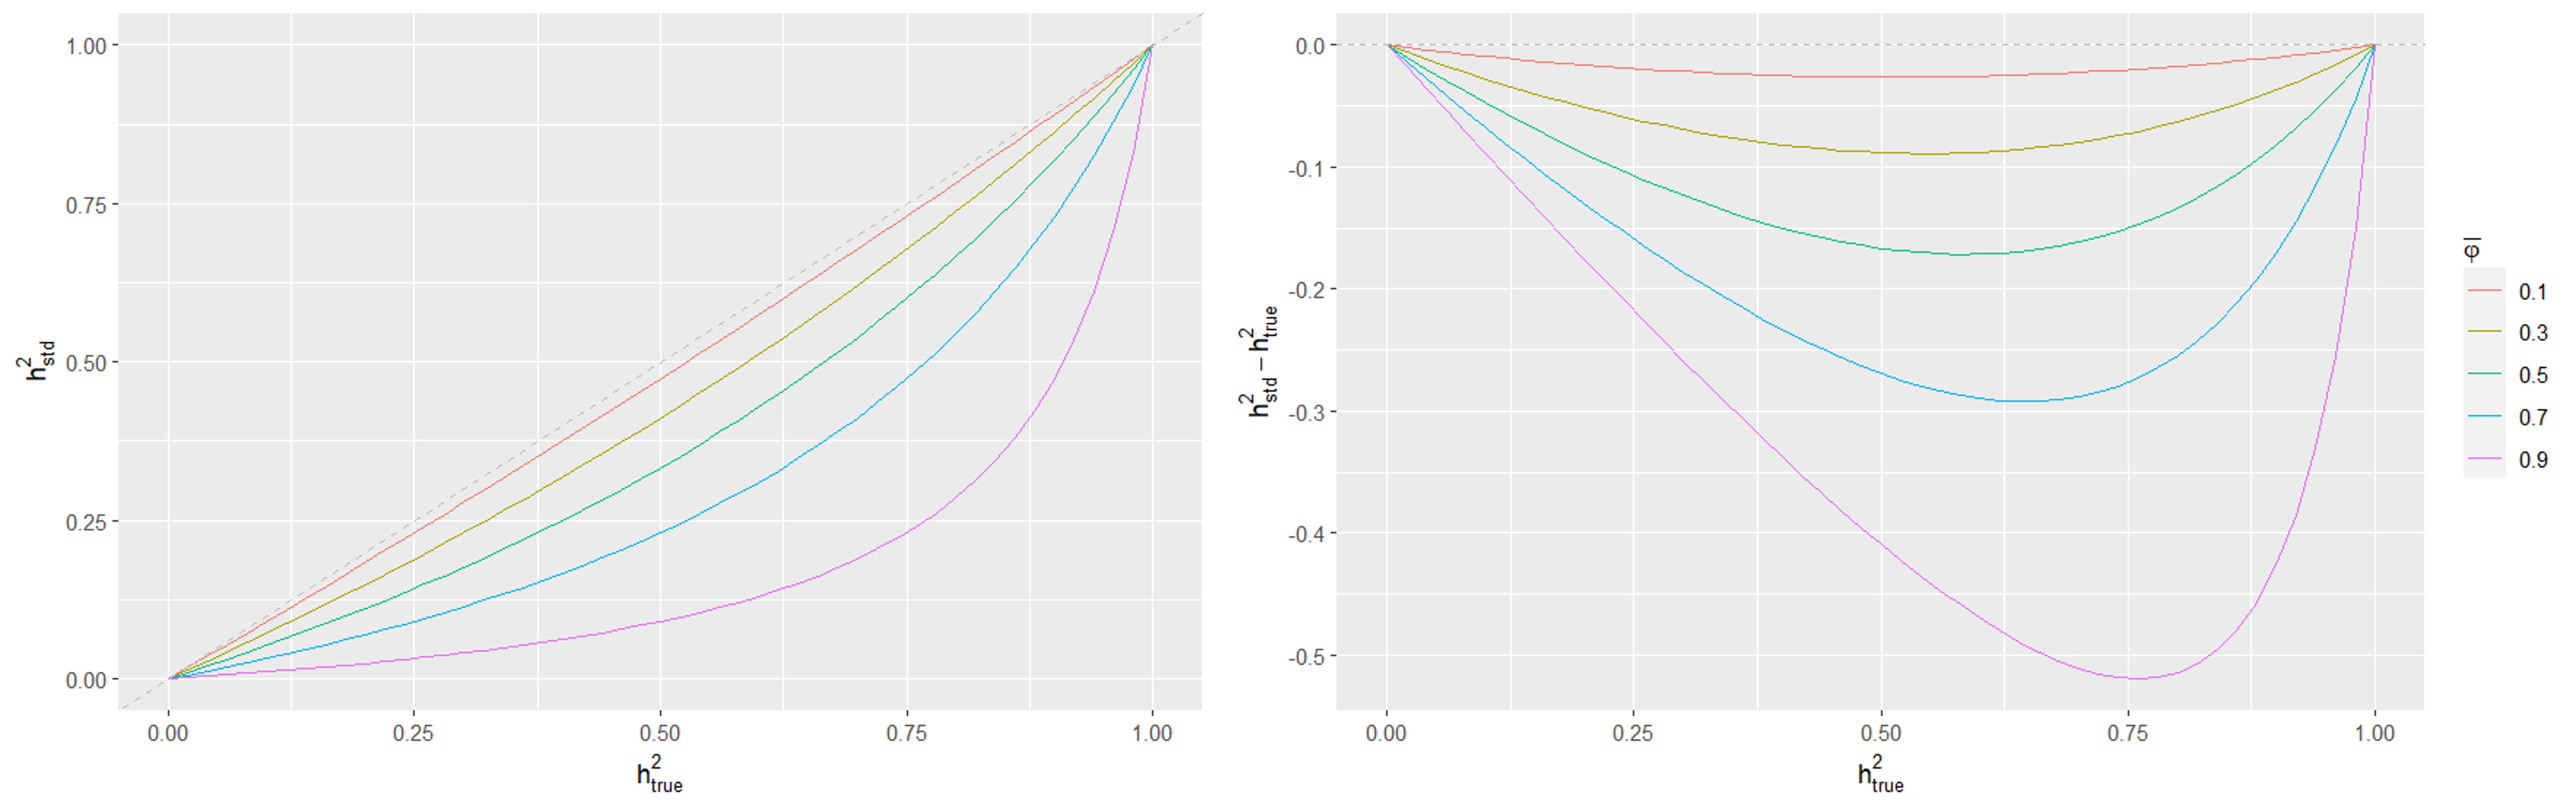
\includegraphics[width=\textwidth]{data/h_both.png}
  \caption{
    {\bf Relationship between the true heritability and biased estimates.}
    The left one plots the relationship between biased estimates and the true heritability, while the right one plots the relationship between the bias and true heritability.
    }
  \label{fig:h}
\end{figure}


\subsection{Software}

Kinship estimates based on the Popkin method are computed using the popkin R package, while standard MOR kinship estimates are obtained with GCTA (version 1.93.2beta). All other kinship estimators are calculated using the popkinsuppl R package. Plink (version 1.90 and 2.00a3LM) is used to process genotype data.


\subsection{Simulations}
To characterize the effect of kinship estimator bias in heritability estimation, we use simulated genotypes and traits and estimate kinship matrices from these genotypes. In particular, we consider the true kinship matrix of the simulation, the unbiased popkin estimator in \cref{eq:popkin}, the standard
kinship estimator in \cref{eq:kinship_std_rom} and \cref{eq:kinship_std_mor}. Each scenario was replicated 50 times, in each case producing a new genotype matrix.

To further explore how rare variants affect kinship estimation and trait simulations, we use genotypes from the 1000 Genome project and simulate traits using different filters ($maf=\{0,0.01,0.05\}$), and estimate the kinship matrix using genotypes based on different filters ($maf=\{0,0.01,0.05\}$) as well. 

\subsubsection{Trait simulation algorithm}

Suppose the genotype matrix $\mathbf{X}$ is available, and we have fixed values for the number of causal loci $m_1$, the trait mean, variance scale, and heritability ($\mu, \sigma^2, h^2$).
The goal is to choose the intercept $\alpha$ and draw random effect sizes $\mathbf{\beta}$ that result in the desired trait parameters.
First we randomly select $m_1$ loci to be causal, and subset the genotype matrix $\mathbf{X}$ and ancestral allele frequency vector $\mathbf{p}$ so that from this point on they contain only those causal loci (they now have dimensions $m_1 \times n$ and length $m_1$, respectively).

Below we divide the algorithm into two steps: (1) scaling the effect sizes, and (2) centering the trait.
Each step forks into two cases: whether the true ancestral allele frequencies $\mathbf{p}$ are known or not (the latter requires a known kinship matrix $\kinMat$).

\textbf{Scaling effect sizes.}
The initial effect sizes $\beta_i$ are drawn independently from a standard normal distribution:
$$
\beta_i \sim \text{N}(0, 1).
$$

First we consider the simpler case of known ancestral allele frequencies $\mathbf{p} = (\pit)$.
The initial genetic variance scale is
$$
\sigma^2_0
=
\sum_{i=1}^{m_1} 2 \pit (1-\pit) \beta_i^2
.
$$
We obtain the desired variance by dividing each $\beta_i$ by $\sigma_0$ (which results in a variance of 1) and then multiply by $h \sigma$ (which results in the desired variance of $h^2 \sigma^2$).
Combining both steps, the update is
$$
\mathbf{\beta}
\leftarrow
\mathbf{\beta} \frac{ h \sigma }{\sigma_0}
.
$$

Now we consider the case of unknown ancestral allele frequencies but known kinship matrix.
First, sample estimates $\mathbf{\hat{p}} = (\pith)$ of the ancestral allele frequencies are constructed from the genotype data as
$$
\pith
=
\frac{1}{2n} \mathbf{1}_n^\intercal \mathbf{x}_i
.
$$
Although this estimator is unbiased ($\E[\mathbf{\hat{p}}] = \mathbf{p}$), the resulting variance estimates of interest $\pith \left( 1-\pith \right)$ are downwardly biased \citep{ochoa_estimating_2021}:
$$
\E \left[ \pith \left( 1-\pith \right) \right]
=
\pit(1-\pit) (1 - \bar{\varphi})
,
$$
where $\bar{\varphi} = \frac{1}{n^2} \mathbf{1}_n^\intercal \kinMat \mathbf{1}_n$ is the mean kinship coefficient in the data.
Therefore the initial genetic variance scale, estimated as
$$
\hat{\sigma}^2_0
=
\sum_{i=1}^{m_1} 2 \pith (1-\pith) \beta_i^2
,
$$
has an expectation of
$$
\E \left[ \hat{\sigma}^2_0 \right]
=
\sigma^2_0 (1 - \bar{\varphi})
.
$$
Therefore, assuming that this additional factor $(1 - \bar{\varphi})$ is known, the update
$$
\mathbf{\beta}
\leftarrow
\mathbf{\beta} \frac{ h \sigma \sqrt{1-\bar{\varphi}} }{\hat{\sigma}_0}
$$
results in the desired variance.

\textbf{Centering the trait.}
Here we consider the problem of selecting the intercept coefficient $\alpha$ that, together with the previous effect size coefficient vector $\mathbf{\beta}$, result in the desired trait mean $\mu$.

When ancestral allele frequencies are known, the trait can be centered precisely.
Given our model, we obtain the desired overall trait mean $\mu$ by choosing the intercept coefficient to be
$$
\alpha 
=
\mu - 2 \mathbf{p}^\intercal \mathbf{\beta}
.
$$

When ancestral allele frequencies are unknown, the solution is to choose the intercept coefficient
\begin{align*}
  \alpha 
  =
  \mu - 2 \hat{\bar{p}} \mathbf{1}_{m_1}^\intercal \mathbf{\beta}
  , \quad\quad
  \hat{\bar{p}}
  =
  \frac{1}{m_1} \mathbf{1}_{m_1}^\intercal \mathbf{\hat{p}}
  =
  \frac{1}{ 2 m_1 n } \mathbf{1}_{m_1}^\intercal \mathbf{X}^\intercal \mathbf{1}_n
  =
  \frac{1}{2} \bar{X}
  ,
\end{align*}
where $\mathbf{1}_{m_1}$ is a length-$m_1$ column vector of ones.
Note that this overal mean allele frequency $\hat{\bar{p}}$ is computed among causal loci only.
This works very well in practice since $\mathbf{\beta}$ is drawn randomly, so it is uncorrelated to $\mathbf{p}$ and therefore
$$
\frac{1}{m_1} \mathbf{p}^\intercal \mathbf{\beta}
=
\frac{1}{m_1} \sum_{i=1}^{m_1} \pit \beta_i
\approx
\left( \frac{1}{m_1} \sum_{i=1}^{m_1} \pit \right)
\left( \frac{1}{m_1} \sum_{i=1}^{m_1} \beta_i \right)
=
\frac{1}{m_1}
\bar{p}
\mathbf{1}_{m_1}^\intercal \mathbf{\beta}
$$
is a good approximation.

Now we discuss why the more obvious naive approach, which would be to center the trait using estimated ancestral allele frequencies as
$
\alpha 
=
\mu - 2 \mathbf{\hat{p}}^\intercal \mathbf{\beta}
,
$
does not work.
This approach is equivalent to centering genotypes at each locus as
$$
\mathbf{y} = \alpha \mathbf{1}_n + \sum_{i=1}^{m_1} (\mathbf{x}_i - 2 \pith \mathbf{1}_n) \beta_i + \mathbf{\epsilon}.
$$
However, this operation introduces a distortion in the covariance of the genotypes \citep{ochoa_estimating_2021}: 
$$
\Cov \left( \mathbf{x}_i - 2 \pith \mathbf{1}_n \right)
=
\pit ( 1 - \pit ) \left( 
\kinMat 
+ \bar{\varphi} \mathbf{1}_n \mathbf{1}_n^\intercal 
- \mathbf{\varphi} \mathbf{1}_n^\intercal 
- \mathbf{1}_n \mathbf{\varphi}^\intercal 
\right),
$$
where $\bar{\varphi}$ is the overall mean kinship, as before, and $\mathbf{\varphi} = \frac{1}{n} \kinMat \mathbf{1}_n$ is a length-$n$ column vector of per-row mean kinship values.
These undesireable distortions propagate to the trait, which we confirmed in simulations (not shown).
%It is not clear how to correct these distortions after centering the trait as shown above.
Note that the intercept version we chose instead does not induce this genotype centering, which prevents the undesireable distortions in the trait covariance.

\subsubsection{Admixture simulation for genotype matrices}

An admixed family is simulated following previous work \citep{yao_limitations_2022}, except here only $K=3$ ancestries are simulated and $F_{ST}=0.3$ for the admixed individuals, which more closely resembles Hispanics and African Americans.
Briefly, our admixture model first simulates $n=1000$ founder individuals with $m=100,000$ loci.
Random ancestral allele frequencies \pit, subpopulation allele frequencies $p_i^{S_u}$, individual-specific allele frequencies $\pi_{ij}$, and genotypes \xij are drawn from this hierarchical model:

\begin{align*}
  \pit
  &\sim
    \text{Uniform}( 0.01, 0.5 )
    , \\
  p_i^{S_u} | \pit
  &\sim
    \text{Beta} \left(
    \pit \left( \frac{1}{ \ft[S_u] } - 1 \right),
    \left( 1 - \pit \right) \left( \frac{1}{ \ft[S_u] } - 1 \right)
    \right)
    , \\
  \pi_{ij}
  &=
    \sum_{u = 1}^K q_{ju} p_i^{S_u}
    , \\
  \xij | \pi_{ij}
  &\sim
    \text{Binomial}(2, \pi_{ij})
    ,
\end{align*}

where this Beta is the Balding-Nichols distribution \citep{balding_method_1995} with mean \pit and variance $\pit \left( 1 - \pit \right) \ft[S_u]$.
We also include family structure in the simulation.
20 generations are generated iteratively.

\subsection{Real data analysis}

We utilize the high-coverage NYGC version of the 1000 Genomes Project \citep{fairley_international_2020} filter using \texttt{plink2} \citep{chang_second-generation_2015}. We retain only autosomal biallelic SNP loci marked with the filter ``PASS''. The final dataset consists of $m=91,784,660$ loci and $n=2,504$ individuals.

San Antonio Family Study (SAMAFS) is a complex pedigree-based study designed to identify low frequency or rare variants influencing susceptibility to T2D, conducted in 20 Mexican American T2D-enriched pedigrees from San Antonio, Texas  \citep{mitchell1996genetic}. We only use exome chip data for the SAMAFS. We use PLINK (version 1.90b4.9) \texttt{--autosome} to exclude all unplaced and non-autosomal variants, and further filter using \texttt{--maf 0.01 --hwe 1e-10} (version 2.00a3LM). The final dataset consists of $m=36,293$ loci and $n=914 $ individuals. We also include pedigree information for the estimation of kinship matrix for this data set. We adjust for age and sex in the heritability estimate.

Hispanic Community Health Study / Study of Latinos (HCHS/SOL) is a multi-center study in Hispanic/Latino populations recruited through four centers in Miami, San Diego, Chicago, and the Bronx New York \citep{sorlie2010design}. Similarly, we filter genotypes using PLINK (version 2.00a3LM) \texttt{--maf 0.01 --hwe 1e-10}. The final dataset consists of $m=1,656,020 $ loci and $n=11,721 $ individuals. We adjust for age and sex in the heritability estimate.

Nephrotic Syndrome (NS) multiethnic cohort is a multi-ancestry study exploring the etiology of nephrotic syndrome \citep{cason2023genetic}. We imputed the genotype and filter genotypes using PLINK (version 2.00a3LM) \texttt{--mac 20}. The final dataset consists of $m=16,605,628  $ loci and $n=1,981  $ individuals. We adjust for sex in the heritability estimate.

\section{Results}

\subsection{Simulation results}
First, we considered a scenario with only population structure, in the absence of family structure. Our findings indicate that only the popkin ROM estimator produces unbiased heritability estimates, whereas all other kinship estimators lead to downwardly biased estimates (\cref{fig:Herit_sim}). To further illustrate the pattern of these biases, we plotted the bias trends for different kinship estimators, which closely align with the theoretical results presented in \cref{fig:h}. Next, we extended our simulations to incorporate both population and family structures. The observed trend in bias remains consistent with the previous scenario; however, the variability in heritability estimates is notably lower.

For the simulation based on data from the 1000 Genomes Project, we set the expected heritability to 0.8. When traits were simulated using all loci, including rare variants, heritability was systematically underestimated across all kinship estimators (\cref{fig:tgp_sim}). However, when traits were simulated using loci filtered to exclude variants with allele frequencies below 0.01 or 0.05, only heritability estimates obtained using the popkin ROM estimator remained unbiased, whereas those based on the Standard MOR estimator continued to underestimate heritability. Furthermore, when kinship matrices were estimated after filtering out a greater proportion of rare variants (maf=0.05), the differences in heritability estimates across kinship estimators became minimal, as the mean kinship values were small in this setting.


\begin{figure}[bp!]
  \centering
  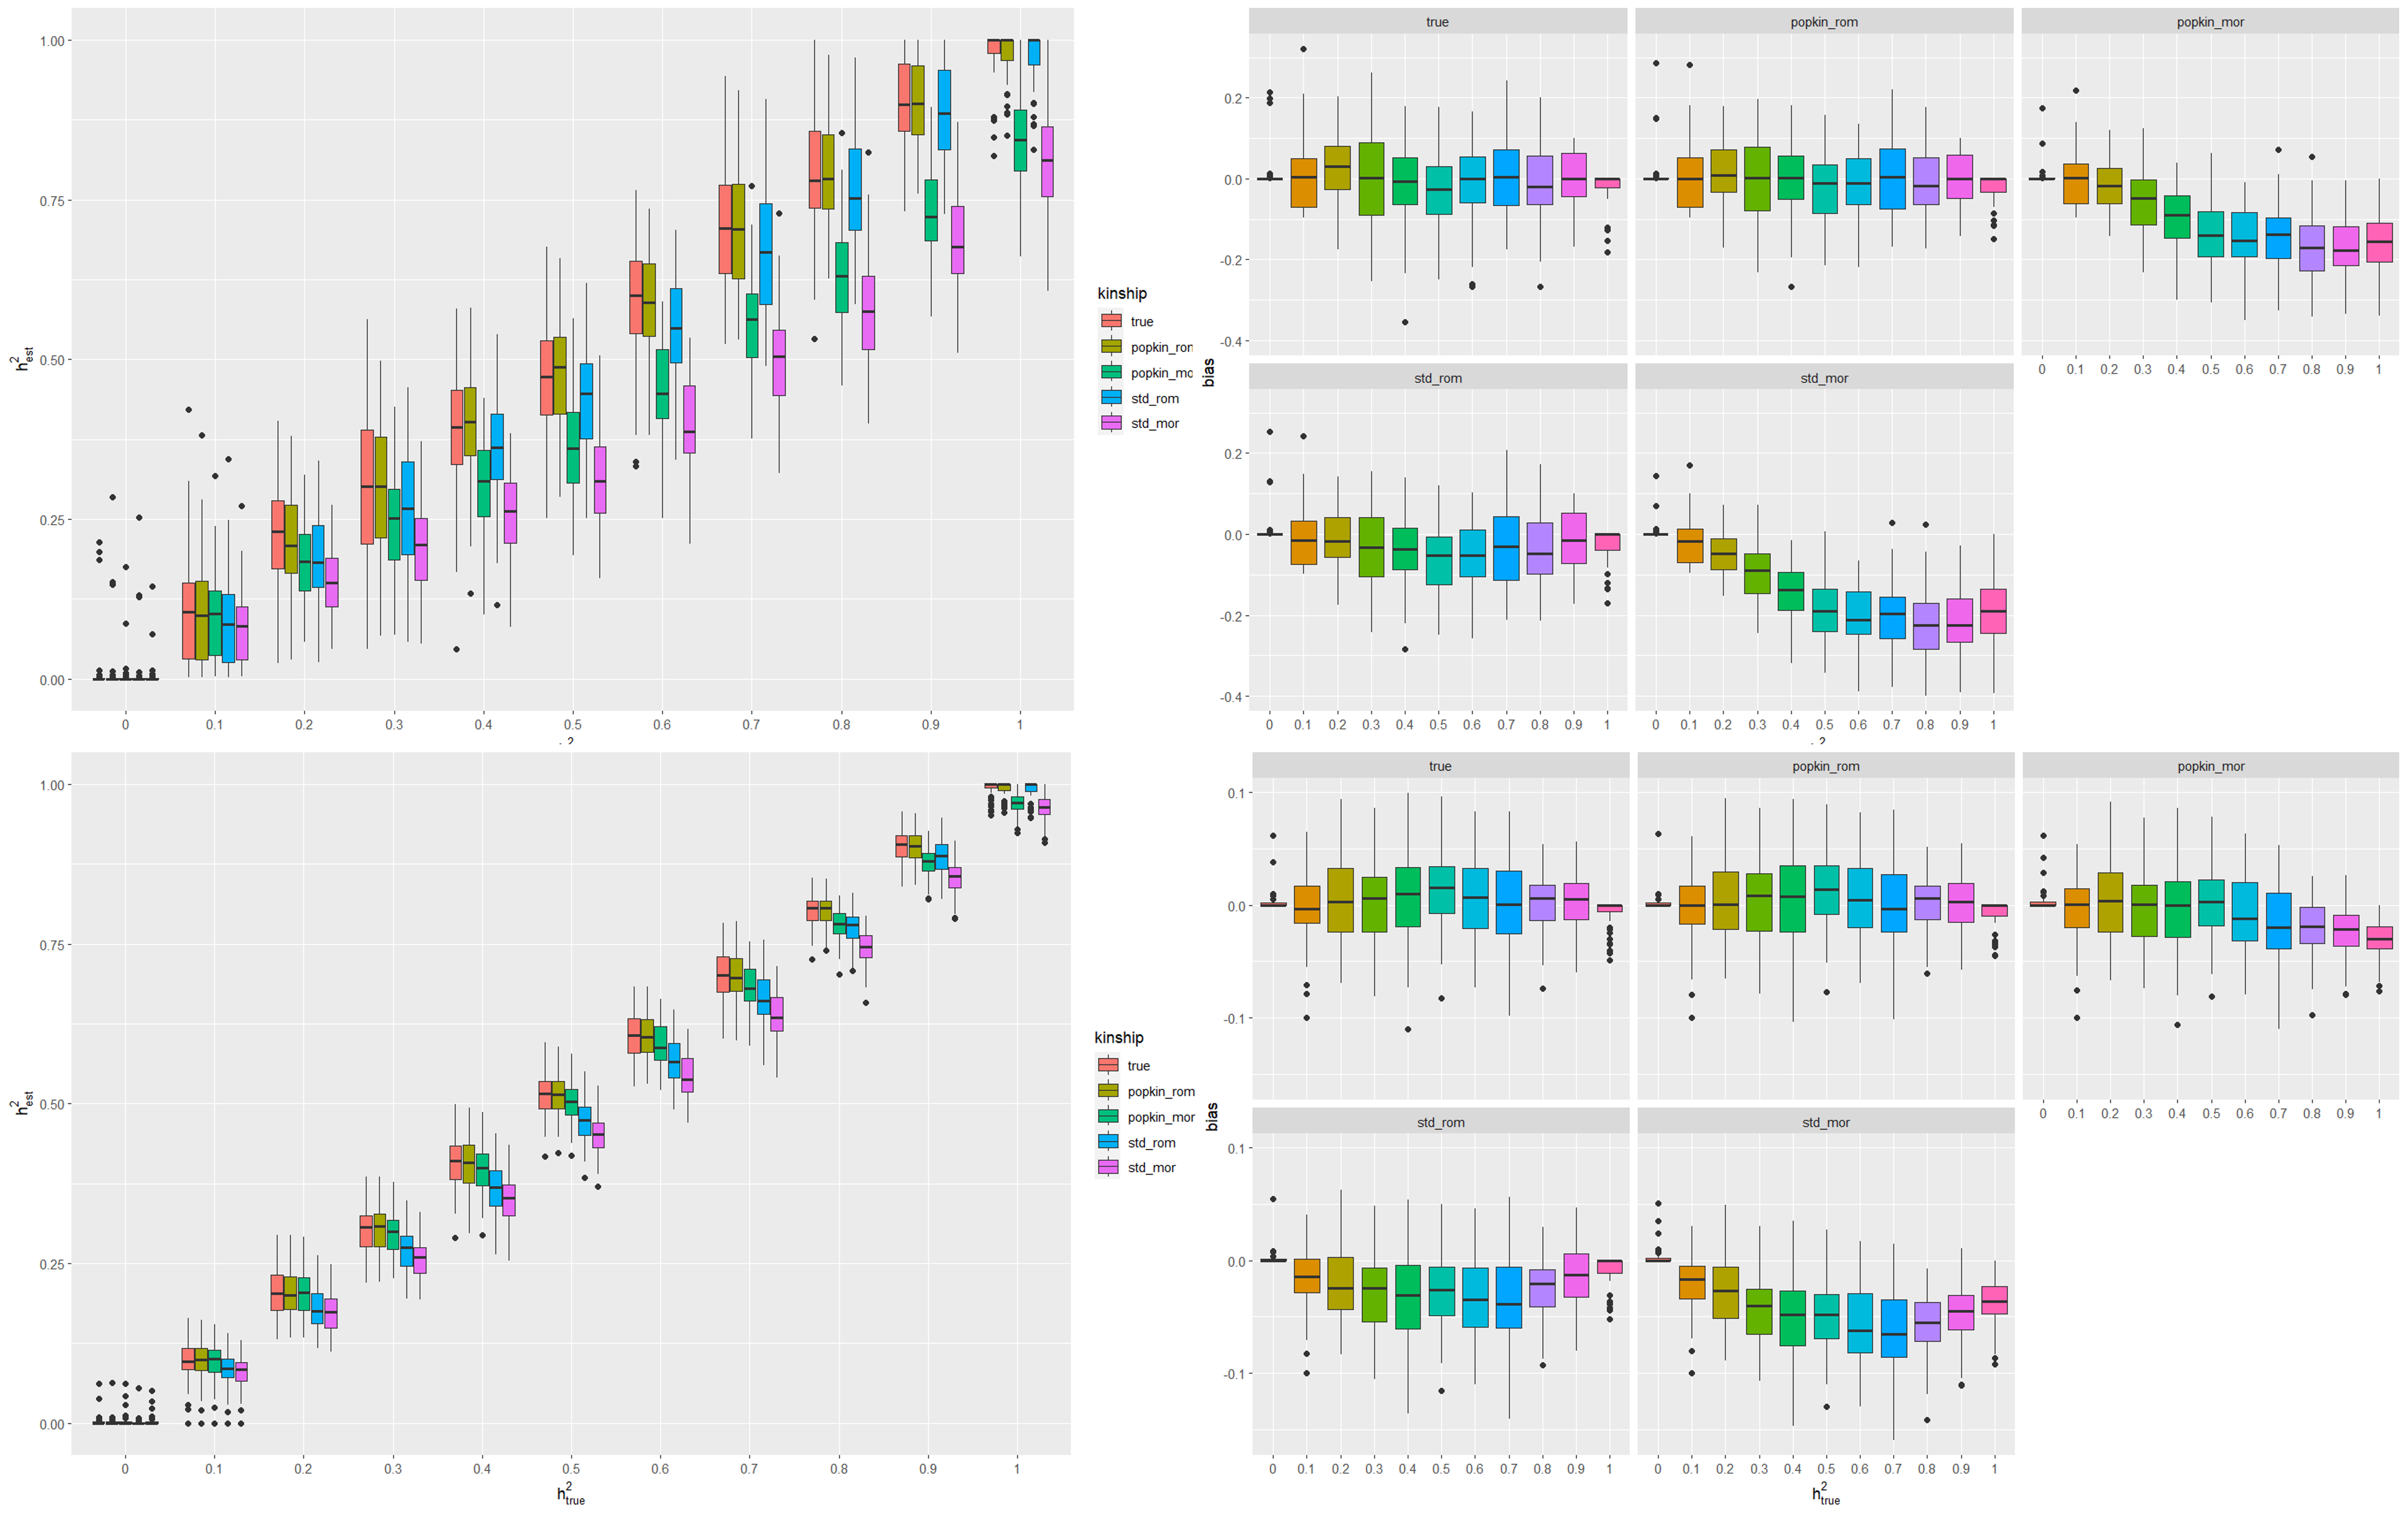
\includegraphics[width=\textwidth]{data/Herit_sim_both.png}
  \caption{
    {\bf Heritability estimation simulation by GCTA with various kinship matrices.}
    The upper and lower rows show simulation results for admixture structure only and admixture plus family structure, respectively.
    }
  \label{fig:Herit_sim}
\end{figure}

\begin{figure}[bp!]
  \centering
  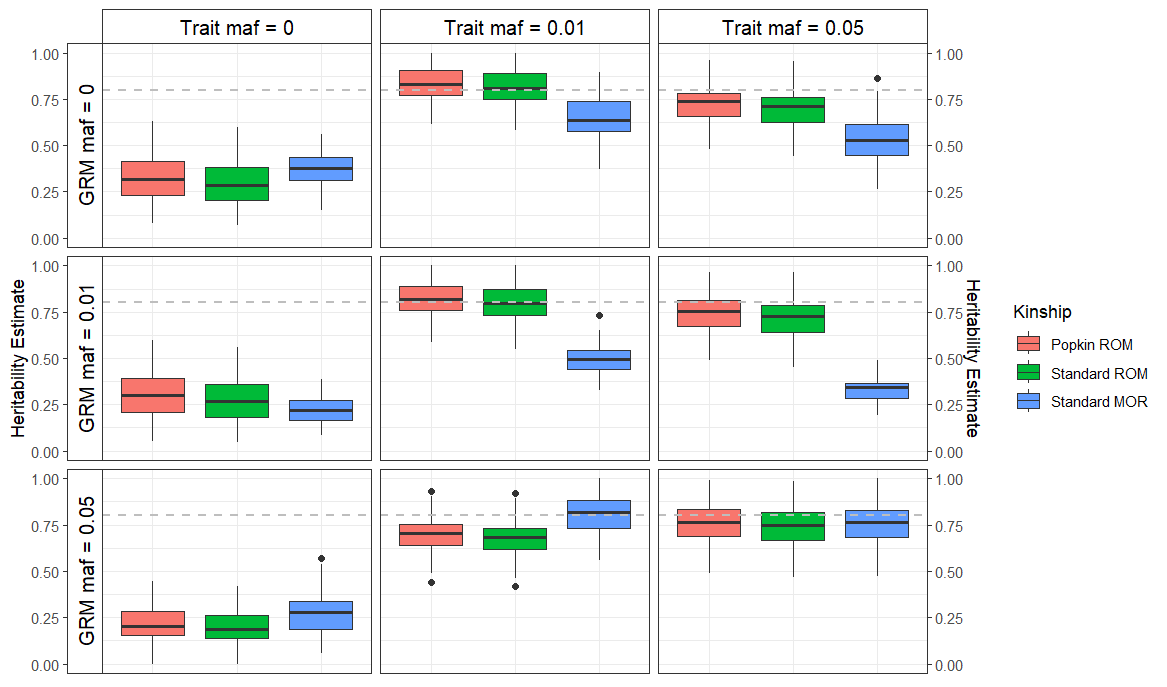
\includegraphics[width=\textwidth]{data/tgp_sim.png}
  \caption{
    {\bf Heritability estimation simulation based on 1000 Genomes Project with various kinship matrices using different rare variants filters.}
    }
  \label{fig:tgp_sim}
\end{figure}


\subsection{Real data applications}
To further validate our findings on real datasets, we estimated heritability using the popkin ROM estimator—an unbiased kinship estimator—and the standard kinship MOR estimator, which is commonly used but known to be biased. These analyses were conducted on three real datasets: the San Antonio Family Study (SAMAFS), the Hispanic Community Health Study/Study of Latinos (HCHS/SOL), and the Nephrotic Syndrome (NS) multiethnic cohort.

For both SAMAFS and HCHS/SOL, heritability estimates derived from the popkin ROM estimator were generally higher across most traits, though some exceptions were observed (\cref{fig:T2D,fig:HCHS}). This discrepancy arises because our theoretical justification in \ref{Estimation bias} applies only to estimators that weight loci consistently (i.e., both ROM or both MOR). These results are consistent with our simulation findings using the 1000 Genomes Project (\cref{fig:tgp_sim}). 

For the NS dataset, all heritability estimates obtained using the popkin ROM estimator were higher than those derived from the standard kinship MOR estimator (\cref{fig:NS}). This can be attributed to the higher mean kinship values in this dataset, which, as demonstrated in \cref{fig:h}, result in greater bias.


% heights, compared with the published papers

\begin{figure}[bp!]
  \centering
  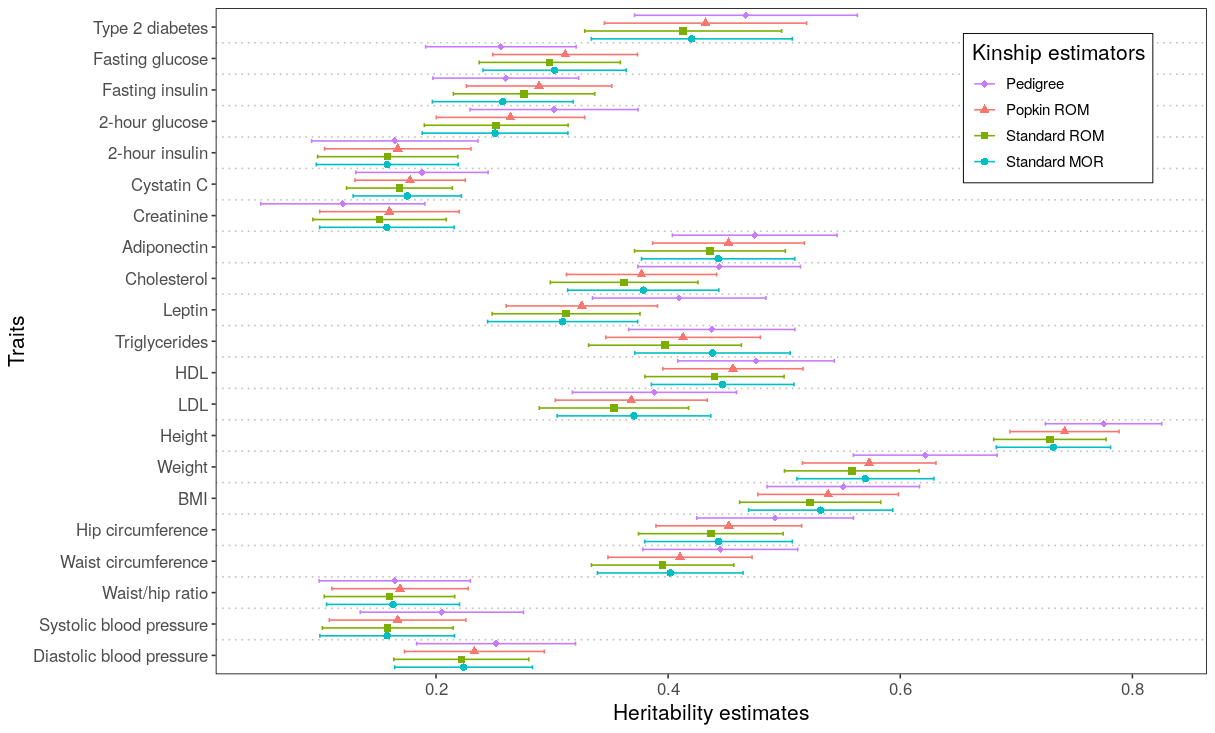
\includegraphics[width=\textwidth]{data/Fig2_T2D_maf001_agesex.png}
  \caption{
    {\bf Heritability estimation on the SAMAFS dataset.}
    The figure shows heritability estimates using pedigree, Popkin ROM, Standard ROM, and Standard MOR kinship estimators on the San Antonio Family Study: Type 2 Diabetes (low mean kinship).
    }
  \label{fig:T2D}
\end{figure}

\begin{figure}[bp!]
  \centering
  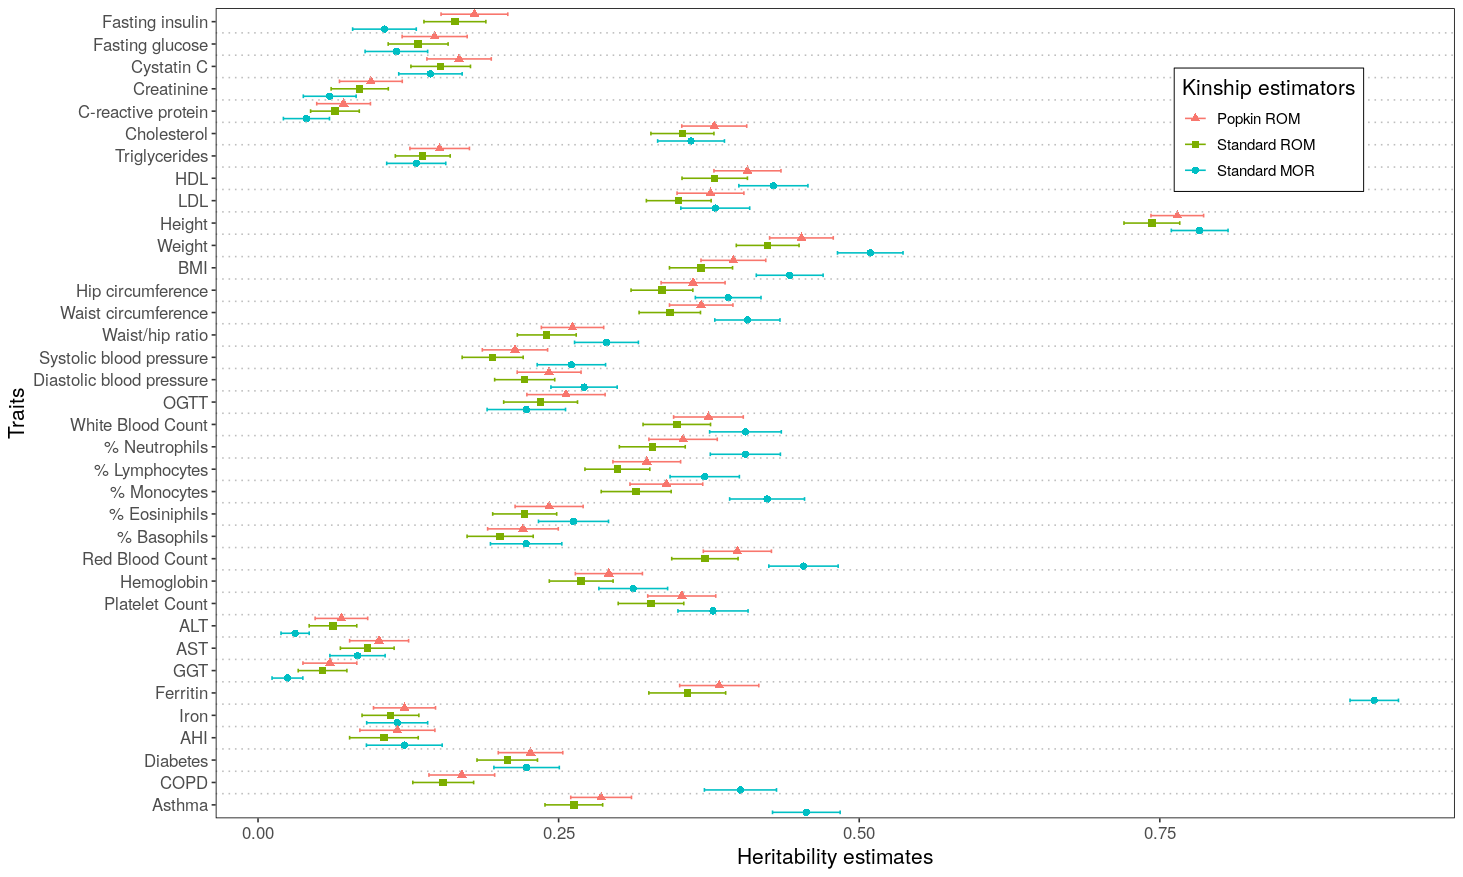
\includegraphics[width=\textwidth]{data/Fig2_HCHS_All_maf001_agesex.png}
  \caption{
    {\bf Heritability estimation on the HCHS/SOL dataset.}
    The figure shows heritability estimates using Popkin ROM, Standard ROM, and Standard MOR kinship estimators on the Hispanic Community Health Study / Study of Latinos (middle mean kinship).
    }
  \label{fig:HCHS}
\end{figure}

\begin{figure}[bp!]
  \centering
  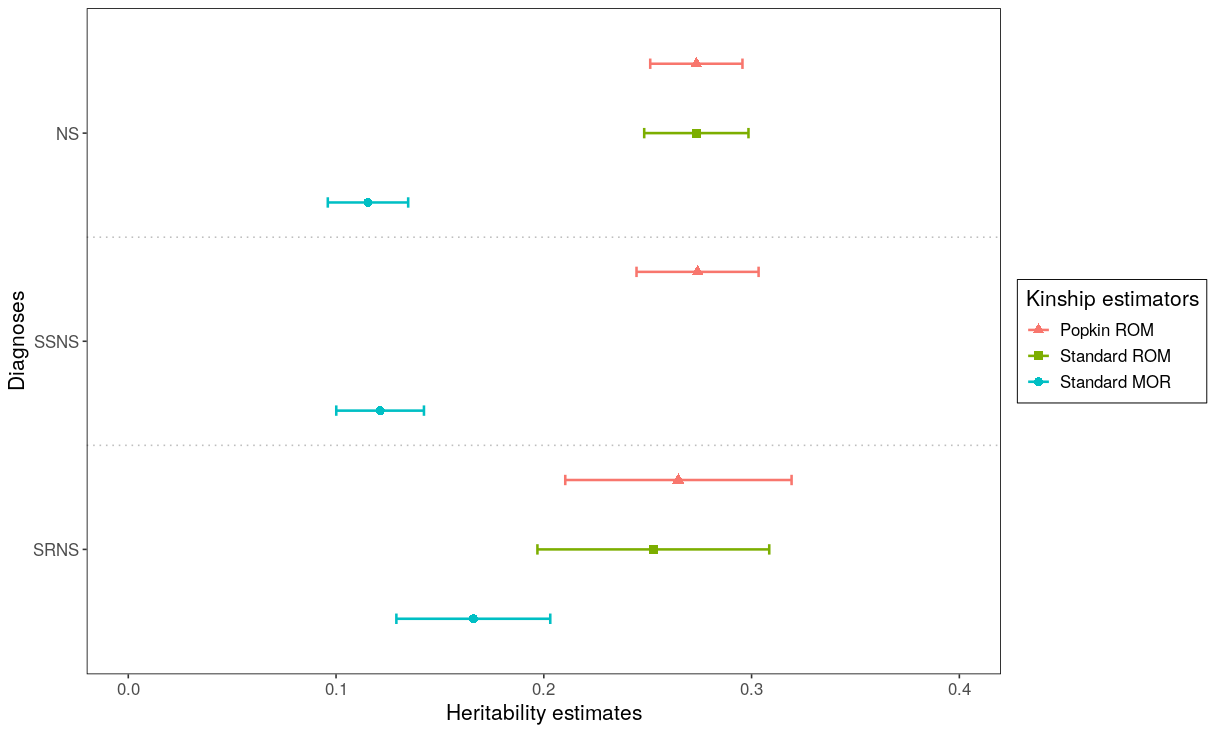
\includegraphics[width=\textwidth]{data/Fig2_NS_sex_array.png}
  \caption{
    {\bf Heritability estimation on the NS dataset.}
    The figure shows heritability estimates using Popkin ROM, Standard ROM, and Standard MOR kinship estimators on the Nephrotic Syndrome: multiethnic cohort (high mean kinship). Note the Standard ROM result for SSNS does not converge, so it is not shown in the figure.
    }
  \label{fig:NS}
\end{figure}



\section{Discussion}

% summary of this whole paper
Previous research has shown that commonly used kinship estimators are biased; however, these biases do not influence association test statistics. In this study, we investigated the impact of kinship estimation bias on heritability and found that this bias propagates to heritability estimation. Specifically, we observed that the Standard kinship estimator (ROM) systematically underestimates heritability, while the bias introduced by the MOR estimators depends on the presence of rare variants.


% ROM and MOR, 1000 genome results
% rare variants simulation, and how it affects MOR

Based on our simulation and real data analysis, the bias between the standard ROM and popkin ROM estimators is evident, with the magnitude of the differences depending on the mean kinship values. However, it remains challenging to quantitatively determine both the direction and the extent of bias between the ROM and MOR versions of the popkin or standard kinship estimators. Based on the formula of the MOR estimator in \cref{eq:kinship_std_mor}, we hypothesize that MOR estimators tend to assign greater weight to the contribution of rare variants. Our simulation studies (\cref{fig:Herit_sim,fig:tgp_sim}) confirm that rare variants may influence the extent of bias in the MOR estimator. Thus, the relationship of heritability using different kinship estimators can be characterized in \cref{fig:est_relationship}.

Directly simulating rare variants is difficult; therefore, in our initial simulation (\cref{fig:Herit_sim}), we primarily generated common variants. Under these conditions, only the popkin ROM estimator produced unbiased heritability estimates, whereas heritability estimates derived from the MOR estimators consistently exhibited downward bias, as further confirmed in the second and third columns of \cref{fig:tgp_sim}.

To simulate traits influenced by rare variants, we utilized genotype data from the 1000 Genomes Project. When traits were generated based on rare variants, we observed that all kinship estimators led to an underestimation of heritability. The heritability of traits affected by rare variants remains a theoretically underdeveloped area, necessitating further research (Some ref papers..). In practical applications, as demonstrated by our real data analysis, certain traits are influenced by rare variants, which may explain why heritability estimates obtained using the popkin ROM are lower than those obtained using the standard MOR estimator.

% San Antonio Family Study pedigree
For the San Antonio Family Study (SAMAFS), pedigree information was available, allowing us to estimate the kinship matrix based on pedigree data and subsequently obtain heritability estimates. Our results indicate that heritability estimated using the pedigree-based kinship matrix is upwardly biased compared to estimates obtained with the popkin ROM estimator. This bias arises because pedigree-derived kinship matrices do not account for cryptic relatedness, leading to inflated heritability estimates. Some research found that studies based on close relatives and family tend to lead to a higher heritability (some ref papers).  


% Binary traits
In the Nephrotic Syndrome (NS) multiethnic cohort, the traits are binary (case vs. control). Heritability was initially estimated directly (observed heritability) and subsequently transformed into liability-scale heritability. In our study, although the liability-scaled heritability estimates ranged from 0.1 to 0.3 after transformation, the observed heritability estimates for NS vs. control and SSNS vs. control using the popkin ROM estimator approached 0.99 (Supplement table index here). This is because $\hat{\sigma}^2_e$ converged to nearly zero after several iterations in the GCTA software. These findings suggest that improved algorithms and transformation frameworks may be necessary to ensure accurate heritability estimation for binary traits.

% Conclusion
In this study, we empirically and theoretically examined the impact of kinship estimation bias on heritability estimation, expanding on prior research that identified biases in commonly used kinship estimators. While these biases do not affect association test statistics, our findings show that they propagate to heritability estimates. Specifically, the Standard ROM kinship estimator consistently underestimates heritability, whereas bias in MOR estimators depends on the presence of rare variants. Through simulations and real data analyses, we observed that the extent of Standard MOR estimator bias is influenced by mean kinship values, with rare variants playing a critical role in shaping bias patterns as well. Overall, our study highlights the importance of selecting appropriate kinship estimators in heritability analyses, particularly in structured populations and rare variant studies. These findings provide key insights into the biases inherent in existing kinship estimators and underscore the need for future research to refine estimation methods for more accurate and reliable heritability inference across diverse genetic datasets.






\begin{figure}[bp!]
  \centering
  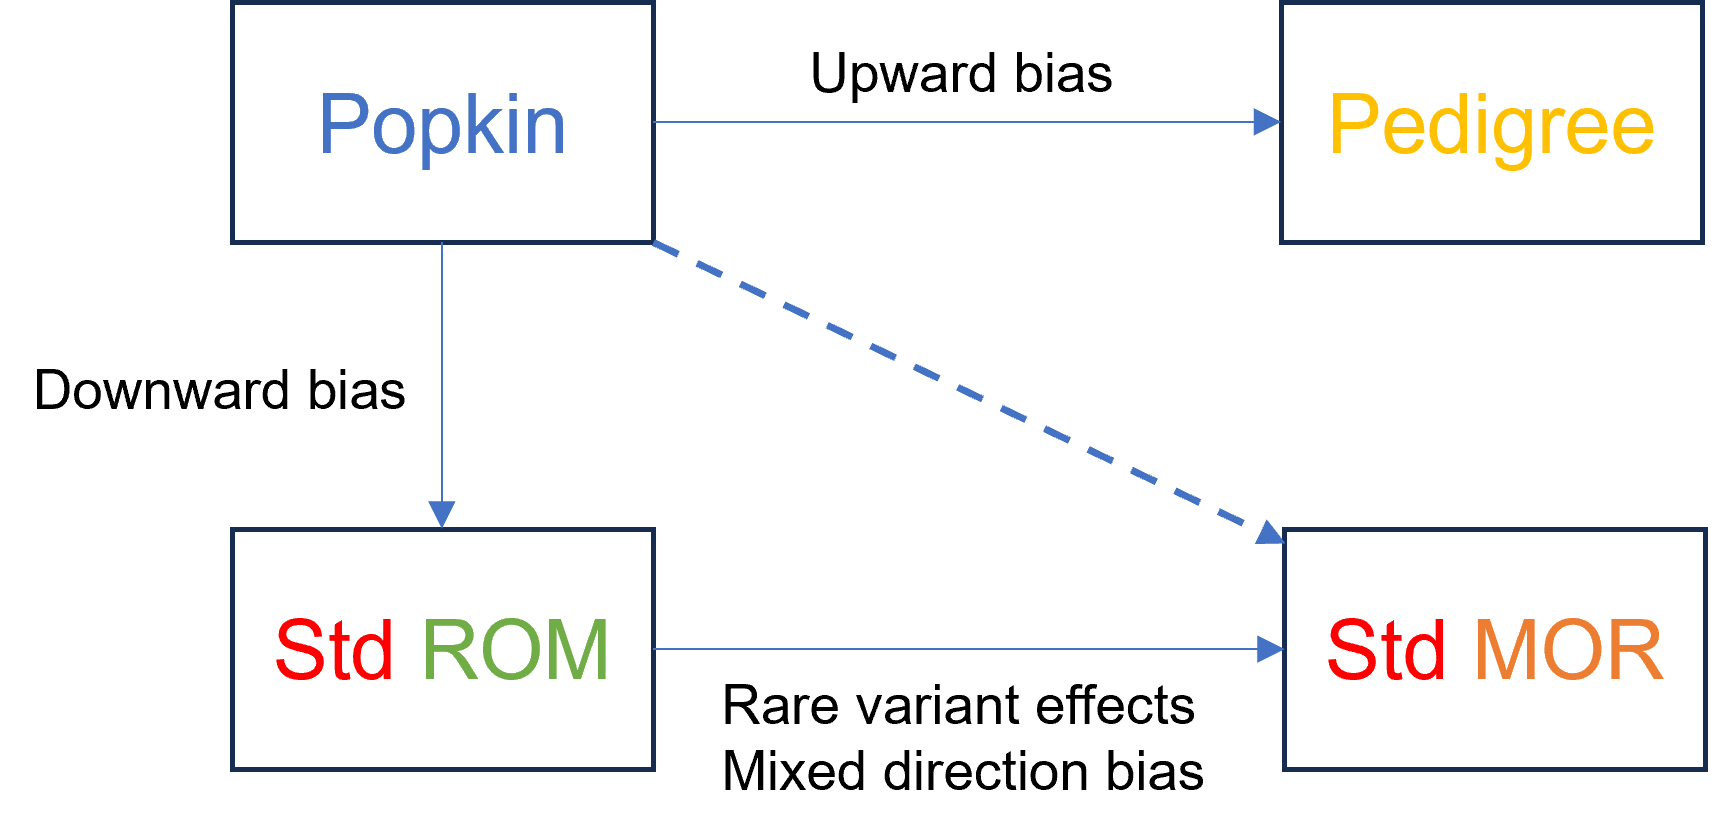
\includegraphics[width=\textwidth]{data/est_relationships.png}
  \caption{
    {\bf Relationships among popkin/standard ROM/MOR estimators.}
    }
  \label{fig:est_relationship}
\end{figure}


\newpage

\printbibliography

\newpage

\beginsupplement

\section{Supplemental Tables and figures}



\begin{table}[h]
  \caption{Heritability for the NS multiethnic cohort}
  \label{tbl:NS_herit_table}
  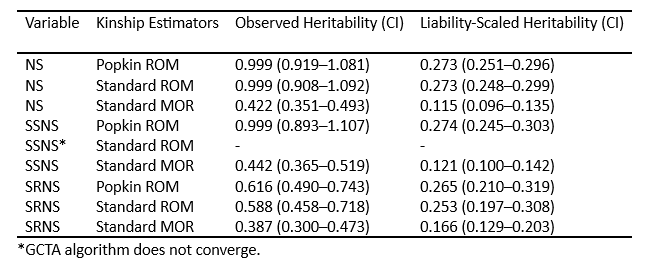
\includegraphics[width=\linewidth]{data/S_table_1_NS_herit.PNG}
\end{table}

\begin{figure}[bp!]
  \centering
  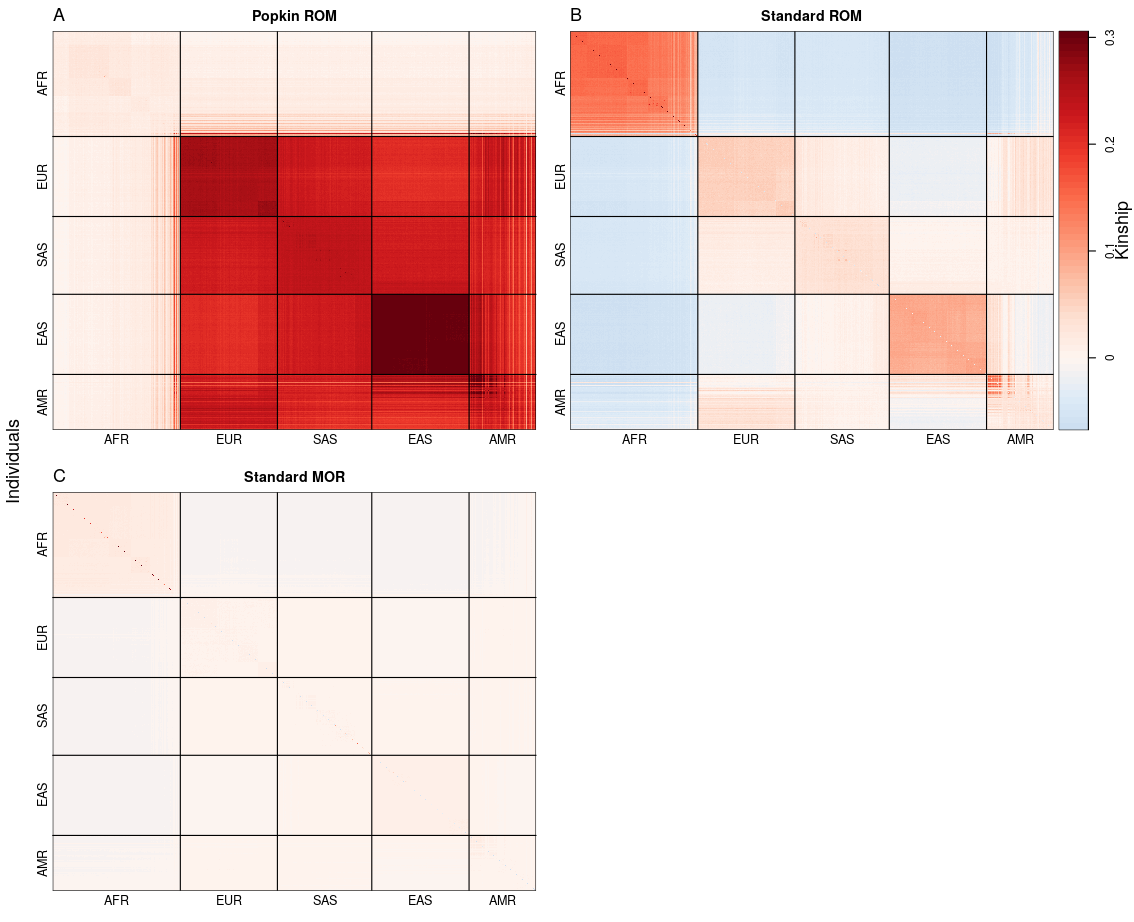
\includegraphics[width=\textwidth]{data/SFig_TGP_kinships.png}
  \caption{
    {\bf Kinships heatmap for the 1000 Genome dataset.}
    }
  \label{fig:TGP_kinships}
\end{figure}

\begin{figure}[bp!]
  \centering
  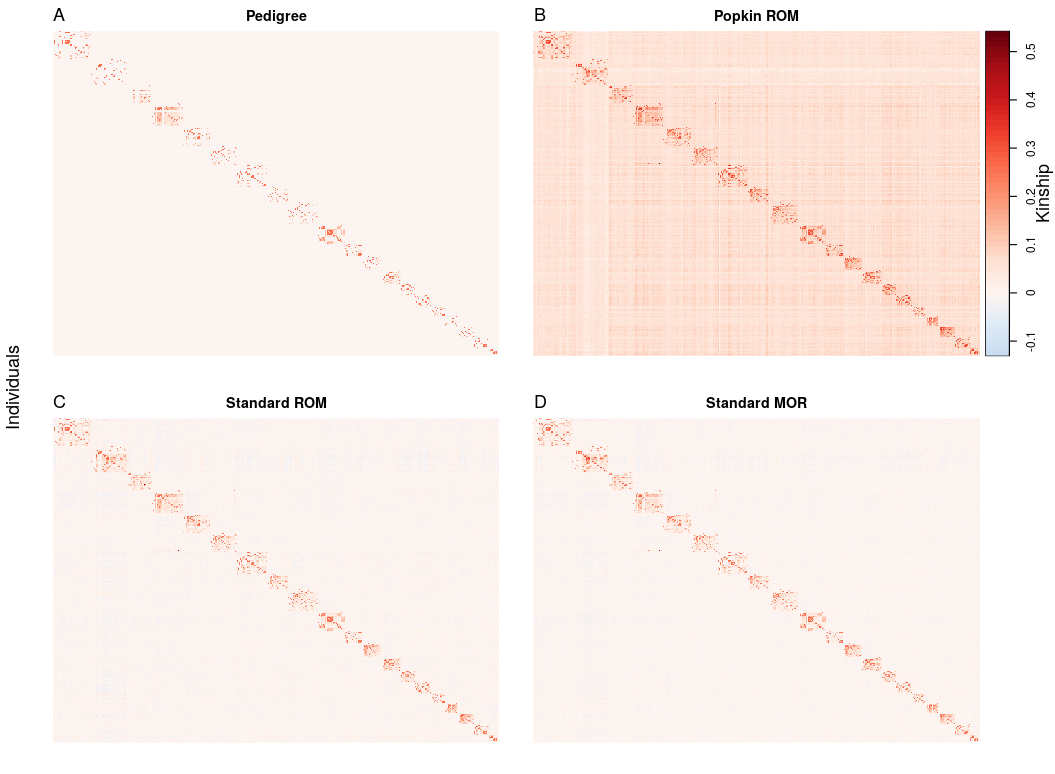
\includegraphics[width=\textwidth]{data/SFig_T2D_kinships.png}
  \caption{
    {\bf Kinships heatmap for the San Antonio Family
Study dataset.}
    }
  \label{fig:T2D_kinships}
\end{figure}

\begin{figure}[bp!]
  \centering
  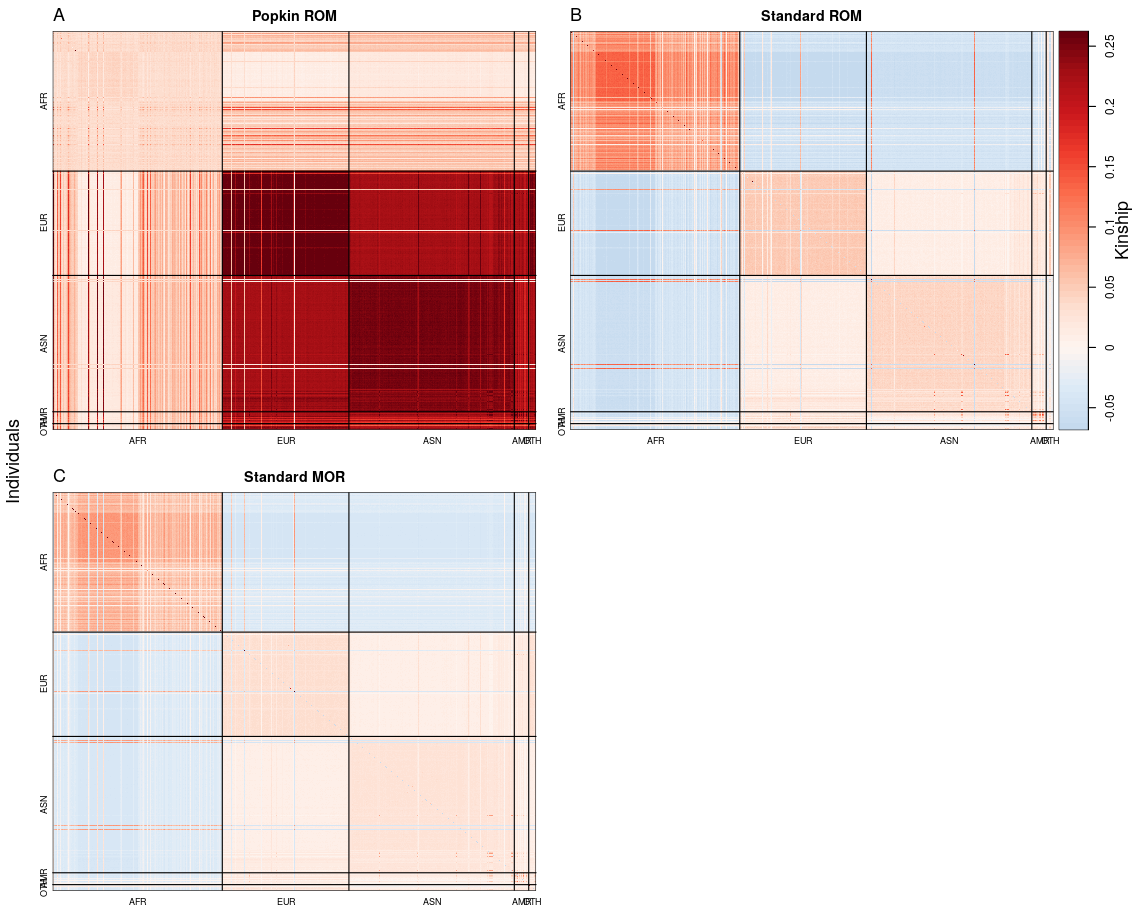
\includegraphics[width=\textwidth]{data/SFig_NS_sex_array_kinships.png}
  \caption{
    {\bf Kinships heatmap for the Nephrotic Syndrome multiethnic cohort dataset.}
    }
  \label{fig:NS_kinships}
\end{figure}

\begin{figure}[bp!]
  \centering
  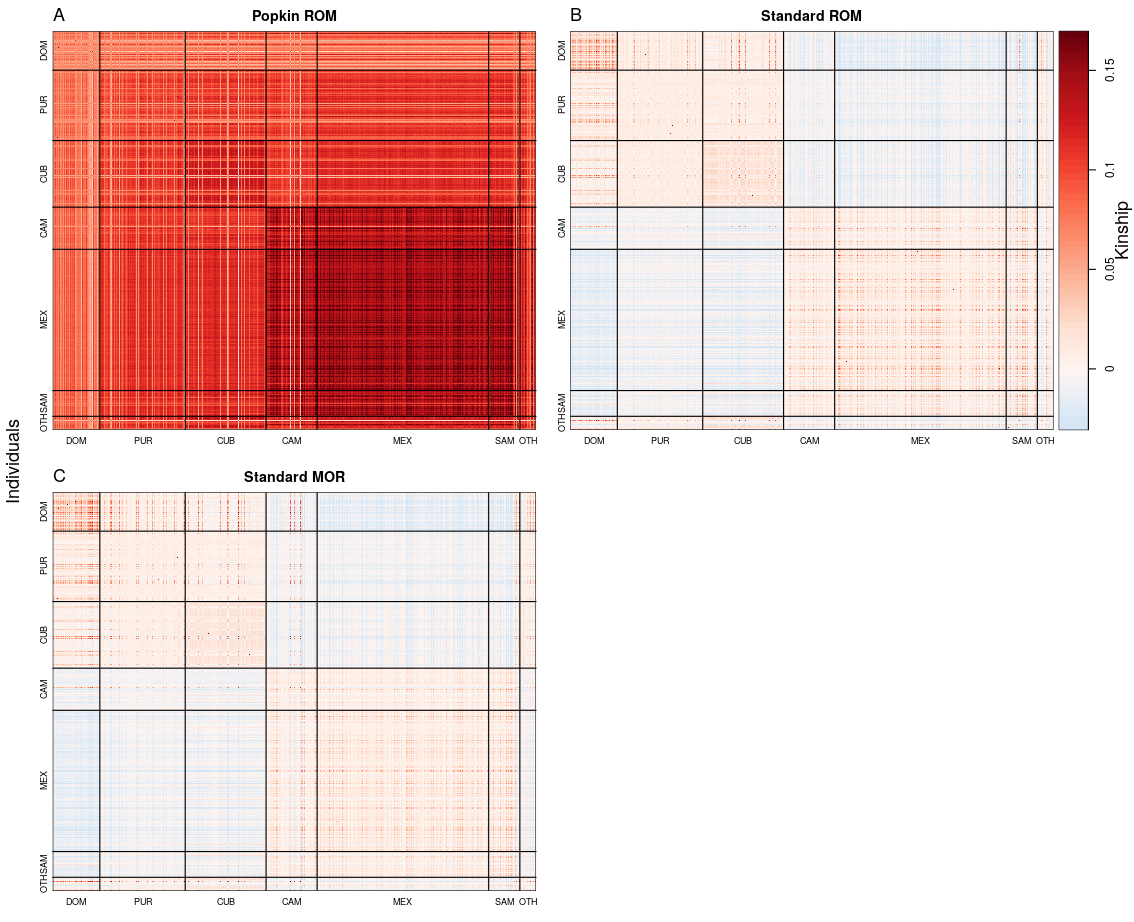
\includegraphics[width=\textwidth]{data/SFig_HCHS_All_maf001_kinships.png}
  \caption{
    {\bf Kinships heatmap for the Hispanic Community Health Study / Study of Latinos dataset.}
    }
  \label{fig:HCHS_kinships}
\end{figure}

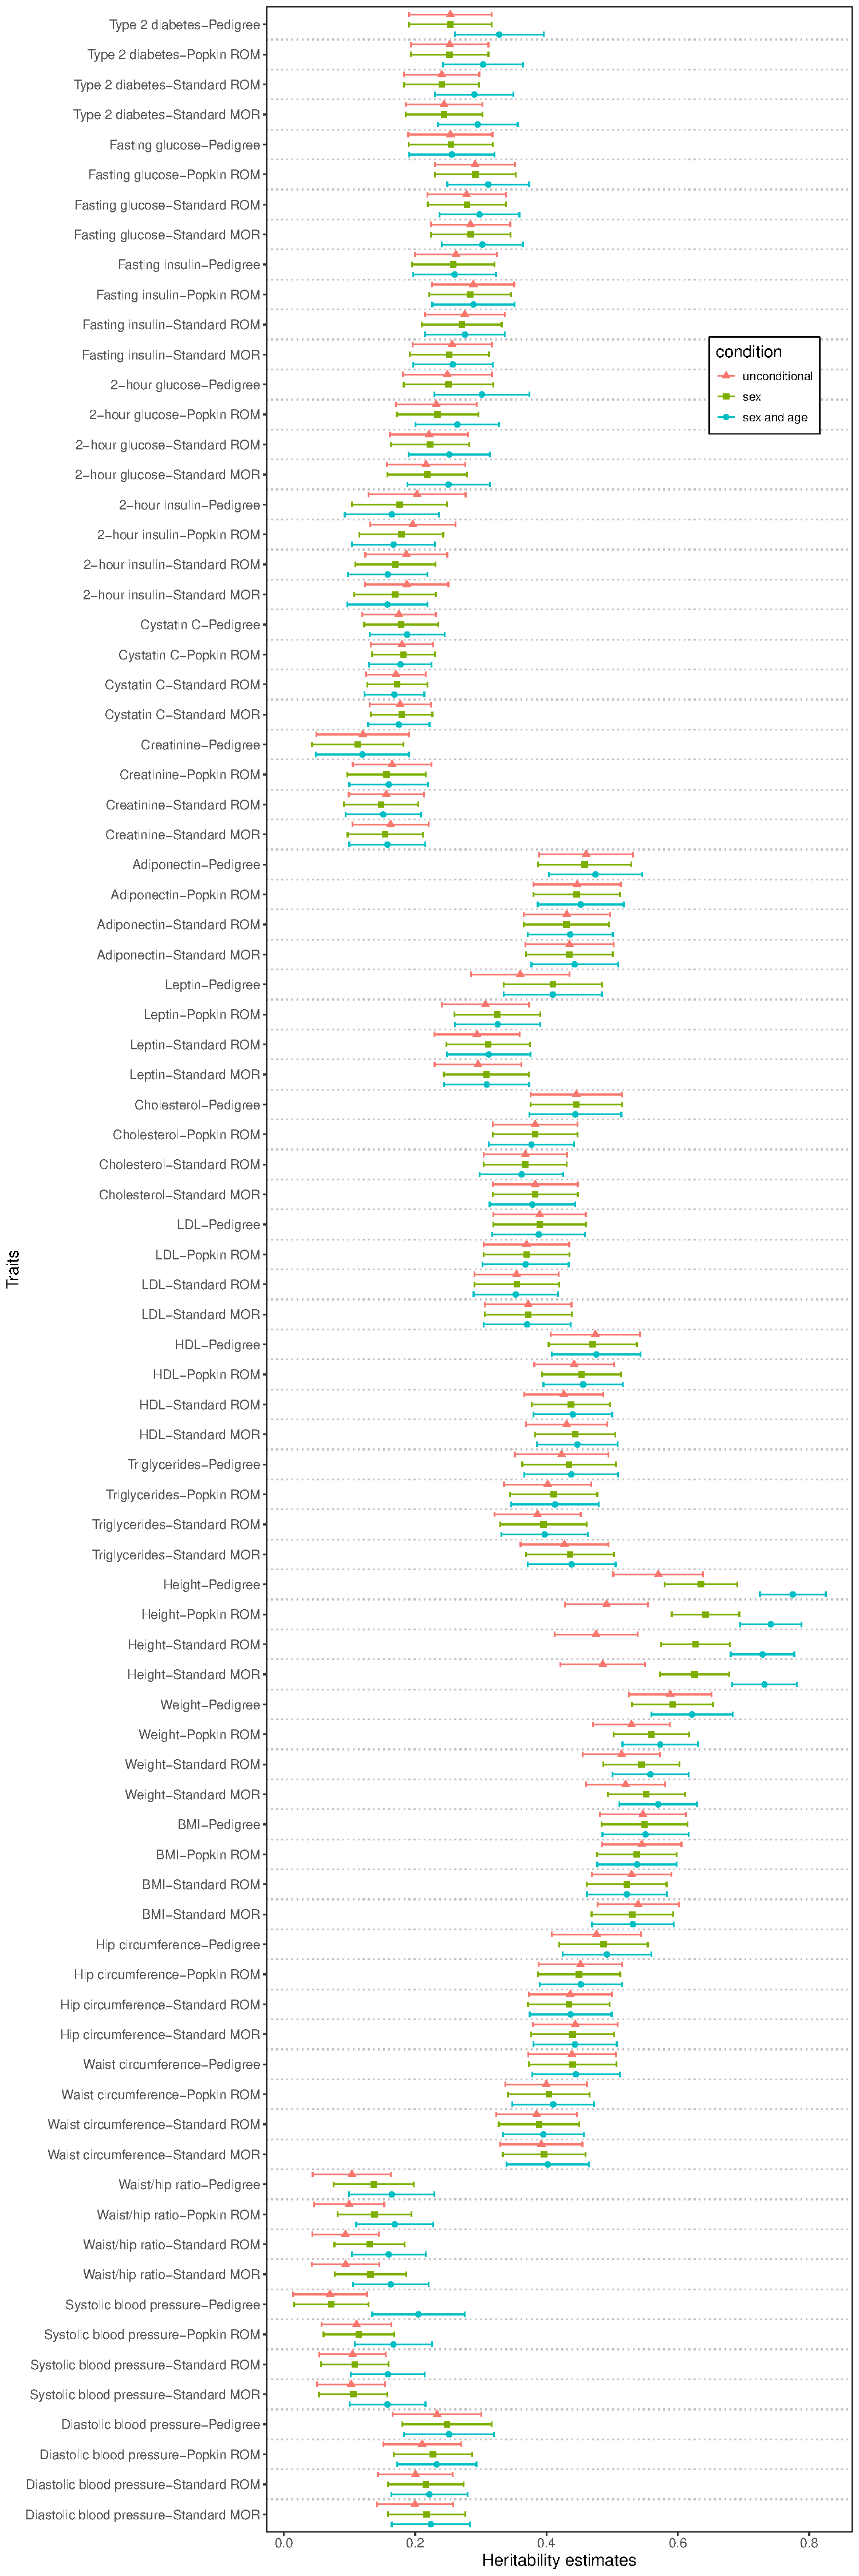
\includepdf[pages=-]{data/SFig_T2D_condition_plot.pdf}

\begin{figure}[bp!]
  \centering
  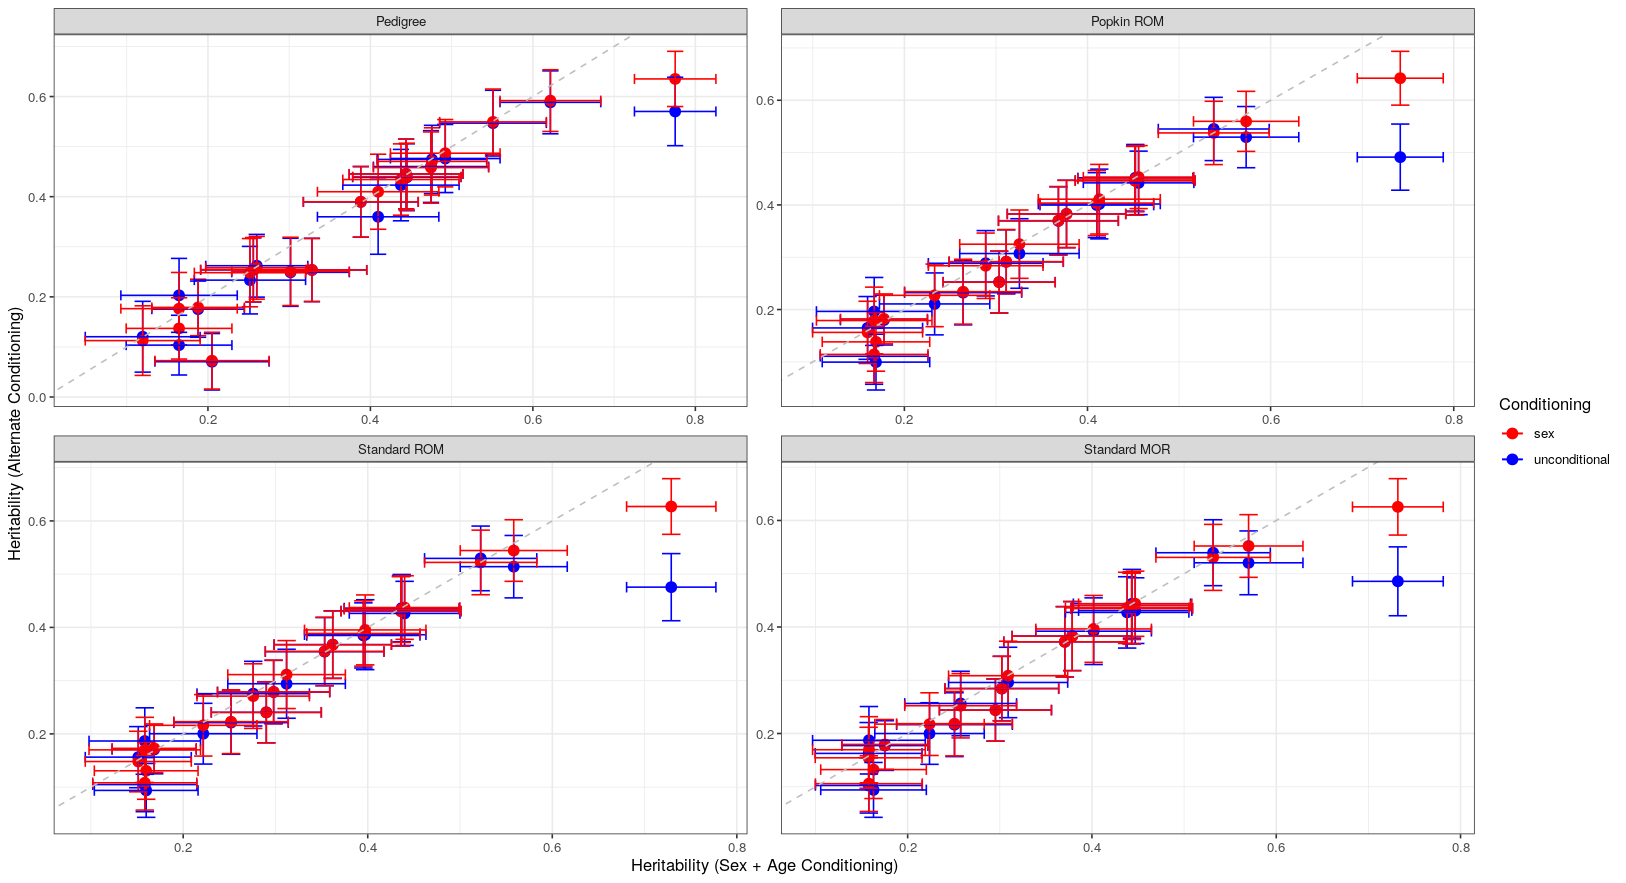
\includegraphics[width=\textwidth]{data/SFig_T2D_condition_compare.png}
  \caption{
    {\bf Compare heritability conditioning on sex and age with other alternative conditioning (unconditional and condition on sex).}
    }
  \label{fig:condition_compare}
\end{figure}



\section{Supplemental ...}



\end{document}
